\documentclass[twoside]{book}

% Packages required by doxygen
\usepackage{fixltx2e}
\usepackage{calc}
\usepackage{doxygen}
\usepackage[export]{adjustbox} % also loads graphicx
\usepackage{graphicx}
\usepackage[utf8]{inputenc}
\usepackage{makeidx}
\usepackage{multicol}
\usepackage{multirow}
\PassOptionsToPackage{warn}{textcomp}
\usepackage{textcomp}
\usepackage[nointegrals]{wasysym}
\usepackage[table]{xcolor}

% Font selection
\usepackage[T1]{fontenc}
\usepackage[scaled=.90]{helvet}
\usepackage{courier}
\usepackage{amssymb}
\usepackage{sectsty}
\renewcommand{\familydefault}{\sfdefault}
\allsectionsfont{%
  \fontseries{bc}\selectfont%
  \color{darkgray}%
}
\renewcommand{\DoxyLabelFont}{%
  \fontseries{bc}\selectfont%
  \color{darkgray}%
}
\newcommand{\+}{\discretionary{\mbox{\scriptsize$\hookleftarrow$}}{}{}}

% Page & text layout
\usepackage{geometry}
\geometry{%
  a4paper,%
  top=2.5cm,%
  bottom=2.5cm,%
  left=2.5cm,%
  right=2.5cm%
}
\tolerance=750
\hfuzz=15pt
\hbadness=750
\setlength{\emergencystretch}{15pt}
\setlength{\parindent}{0cm}
\setlength{\parskip}{3ex plus 2ex minus 2ex}
\makeatletter
\renewcommand{\paragraph}{%
  \@startsection{paragraph}{4}{0ex}{-1.0ex}{1.0ex}{%
    \normalfont\normalsize\bfseries\SS@parafont%
  }%
}
\renewcommand{\subparagraph}{%
  \@startsection{subparagraph}{5}{0ex}{-1.0ex}{1.0ex}{%
    \normalfont\normalsize\bfseries\SS@subparafont%
  }%
}
\makeatother

% Headers & footers
\usepackage{fancyhdr}
\pagestyle{fancyplain}
\fancyhead[LE]{\fancyplain{}{\bfseries\thepage}}
\fancyhead[CE]{\fancyplain{}{}}
\fancyhead[RE]{\fancyplain{}{\bfseries\leftmark}}
\fancyhead[LO]{\fancyplain{}{\bfseries\rightmark}}
\fancyhead[CO]{\fancyplain{}{}}
\fancyhead[RO]{\fancyplain{}{\bfseries\thepage}}
\fancyfoot[LE]{\fancyplain{}{}}
\fancyfoot[CE]{\fancyplain{}{}}
\fancyfoot[RE]{\fancyplain{}{\bfseries\scriptsize Generated by Doxygen }}
\fancyfoot[LO]{\fancyplain{}{\bfseries\scriptsize Generated by Doxygen }}
\fancyfoot[CO]{\fancyplain{}{}}
\fancyfoot[RO]{\fancyplain{}{}}
\renewcommand{\footrulewidth}{0.4pt}
\renewcommand{\chaptermark}[1]{%
  \markboth{#1}{}%
}
\renewcommand{\sectionmark}[1]{%
  \markright{\thesection\ #1}%
}

% Indices & bibliography
\usepackage{natbib}
\usepackage[titles]{tocloft}
\setcounter{tocdepth}{3}
\setcounter{secnumdepth}{5}
\makeindex

% Custom commands
\newcommand{\clearemptydoublepage}{%
  \newpage{\pagestyle{empty}\cleardoublepage}%
}

\usepackage{caption}
\captionsetup{labelsep=space,justification=centering,font={bf},singlelinecheck=off,skip=4pt,position=top}

%===== C O N T E N T S =====

\begin{document}

% Titlepage & ToC
\pagenumbering{alph}
\begin{titlepage}
\vspace*{7cm}
\begin{center}%
{\Large The Neuron project }\\
\vspace*{1cm}
{\large Generated by Doxygen 1.8.13}\\
\end{center}
\end{titlepage}
\clearemptydoublepage
\pagenumbering{roman}
\tableofcontents
\clearemptydoublepage
\pagenumbering{arabic}

%--- Begin generated contents ---
\chapter{Hierarchical Index}
\section{Class Hierarchy}
This inheritance list is sorted roughly, but not completely, alphabetically\+:\begin{DoxyCompactList}
\item \contentsline{section}{Network}{\pageref{class_network}}{}
\item \contentsline{section}{Neuron}{\pageref{class_neuron}}{}
\begin{DoxyCompactList}
\item \contentsline{section}{Excitatory}{\pageref{class_excitatory}}{}
\item \contentsline{section}{Inhibitory}{\pageref{class_inhibitory}}{}
\end{DoxyCompactList}
\end{DoxyCompactList}

\chapter{Class Index}
\section{Class List}
Here are the classes, structs, unions and interfaces with brief descriptions\+:\begin{DoxyCompactList}
\item\contentsline{section}{\textbf{ Excitatory} }{\pageref{class_excitatory}}{}
\item\contentsline{section}{\textbf{ Inhibitory} }{\pageref{class_inhibitory}}{}
\item\contentsline{section}{\textbf{ Network} }{\pageref{class_network}}{}
\item\contentsline{section}{\textbf{ Neuron} }{\pageref{class_neuron}}{}
\end{DoxyCompactList}

\chapter{Class Documentation}
\section{Excitatory Class Reference}
\label{class_excitatory}\index{Excitatory@{Excitatory}}


{\ttfamily \#include $<$Excitatory.\+hpp$>$}

Inheritance diagram for Excitatory\+:\begin{figure}[H]
\begin{center}
\leavevmode
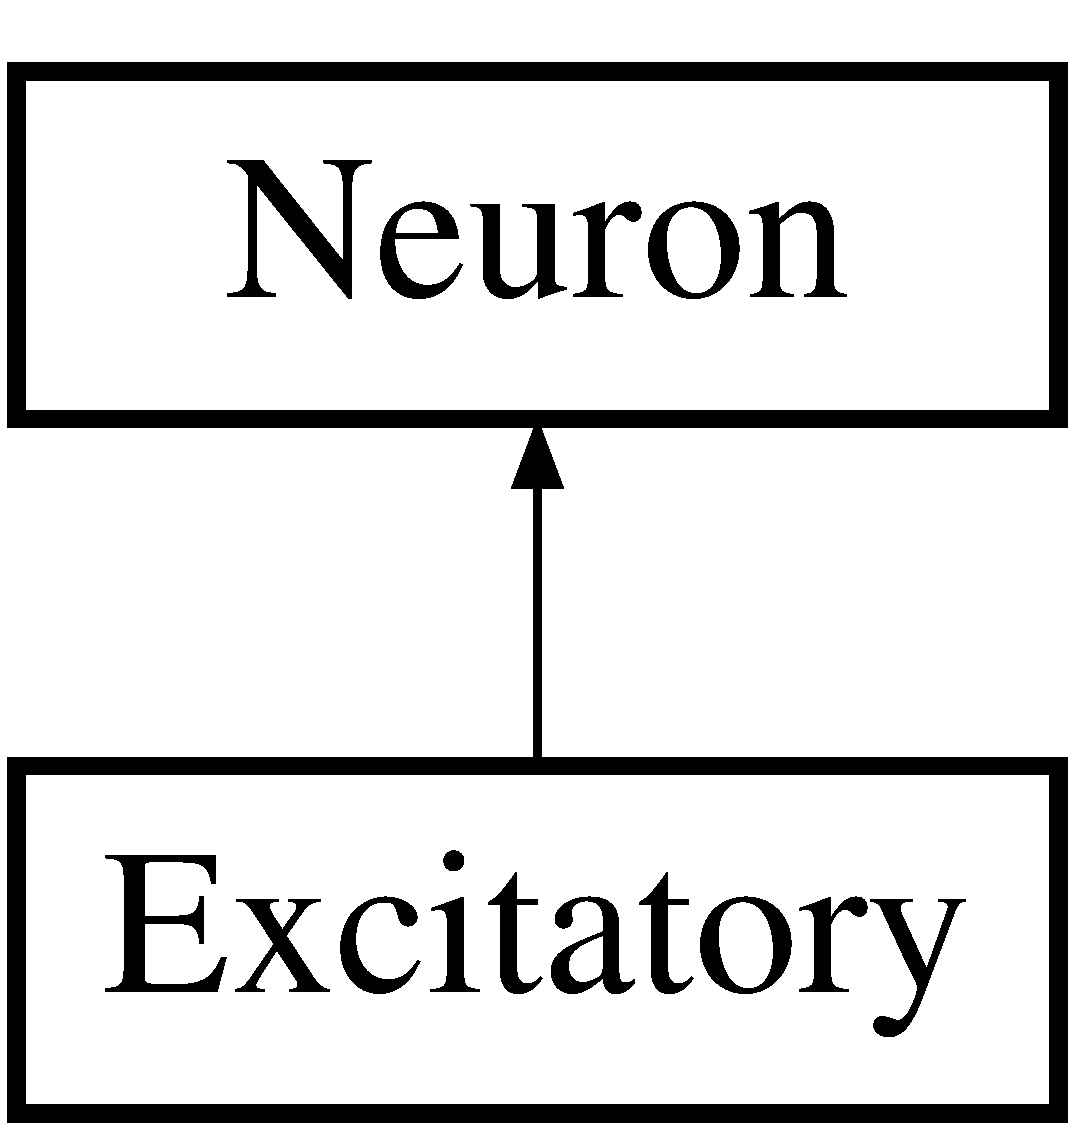
\includegraphics[height=2.000000cm]{class_excitatory}
\end{center}
\end{figure}
\subsection*{Public Member Functions}
\begin{DoxyCompactItemize}
\item 
\textbf{ Excitatory} (unsigned int index)
\begin{DoxyCompactList}\small\item\em The amplitude of the postsynaptic current of an excitatory neuron = 0.\+1 mV. \end{DoxyCompactList}\end{DoxyCompactItemize}
\subsection*{Additional Inherited Members}


\subsection{Detailed Description}
The \doxyref{Excitatory}{p.}{class_excitatory} class which is a subclass of \doxyref{Neuron}{p.}{class_neuron} 

\subsection{Constructor \& Destructor Documentation}
\mbox{\label{class_excitatory_a750ac8872307df0c128801df05aaba46}} 
\index{Excitatory@{Excitatory}!Excitatory@{Excitatory}}
\index{Excitatory@{Excitatory}!Excitatory@{Excitatory}}
\subsubsection{Excitatory()}
{\footnotesize\ttfamily Excitatory\+::\+Excitatory (\begin{DoxyParamCaption}\item[{unsigned int}]{index }\end{DoxyParamCaption})}



The amplitude of the postsynaptic current of an excitatory neuron = 0.\+1 mV. 

Constructor calls the constructor of \doxyref{Neuron}{p.}{class_neuron} with index and the amplitude of the postsynaptic current for the excitatory neurons (Je) = 0.\+1 mV 
\begin{DoxyParams}{Parameters}
{\em index} & the index of the excitaory neuron goes from 0 to nb\+\_\+excit-\/1(10000-\/1)\\
\hline
\end{DoxyParams}
Constructor The index of the excitatory neuron should be between 0 and nb\+\_\+excit -\/1 (10000-\/1)

The documentation for this class was generated from the following files\+:\begin{DoxyCompactItemize}
\item 
Excitatory.\+hpp\item 
Excitatory.\+cpp\end{DoxyCompactItemize}

\section{Inhibitory Class Reference}
\label{class_inhibitory}\index{Inhibitory@{Inhibitory}}
Inheritance diagram for Inhibitory\+:\begin{figure}[H]
\begin{center}
\leavevmode
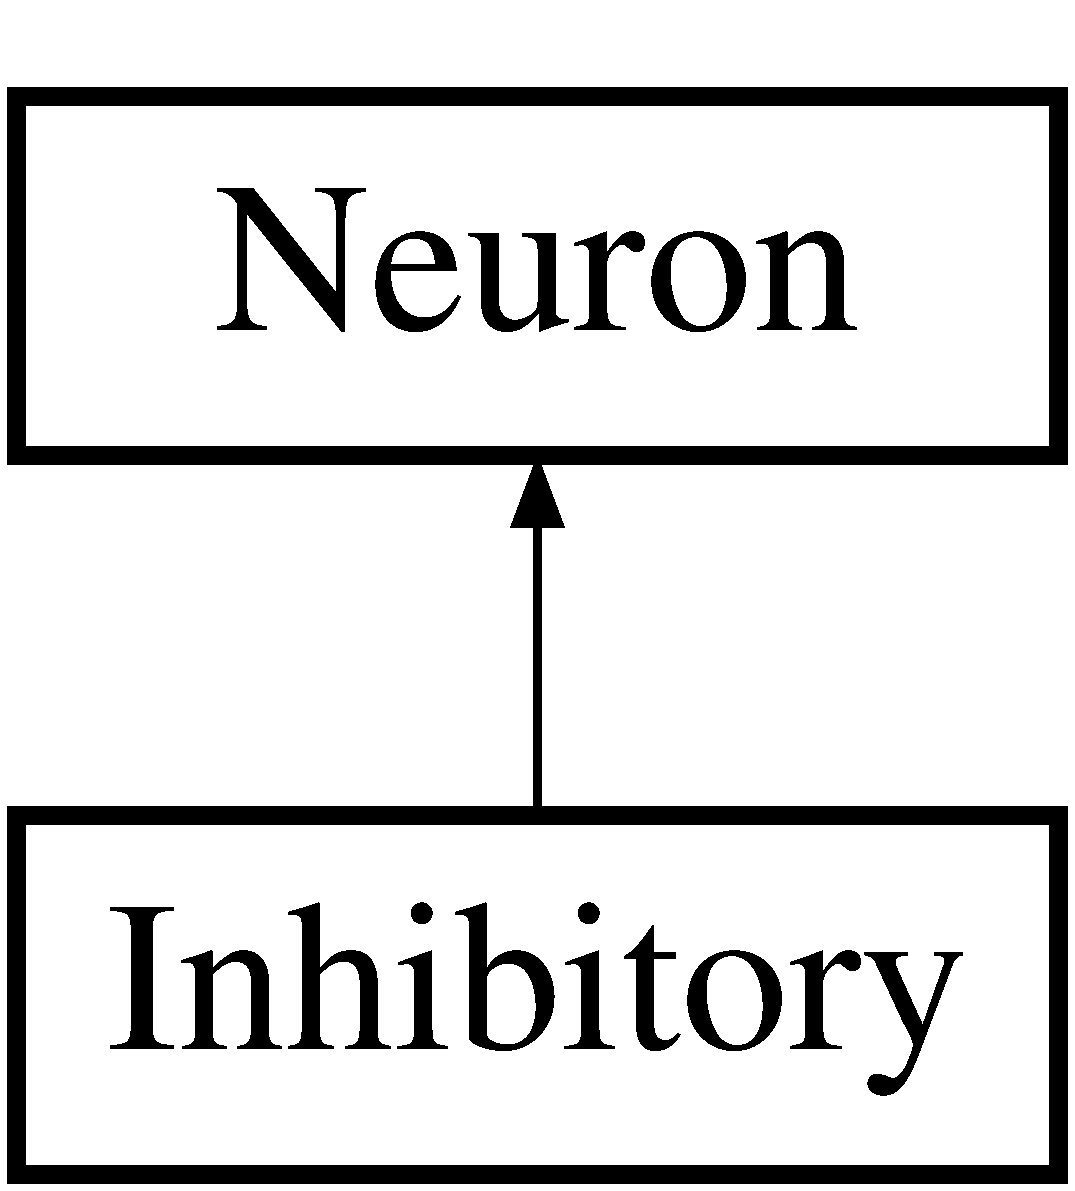
\includegraphics[height=2.000000cm]{class_inhibitory}
\end{center}
\end{figure}
\subsection*{Public Member Functions}
\begin{DoxyCompactItemize}
\item 
\textbf{ Inhibitory} (unsigned int index)
\begin{DoxyCompactList}\small\item\em The amplitude of the postsynaptic current of an inhibitory neuron = 0.\+5 mV. \end{DoxyCompactList}\end{DoxyCompactItemize}
\subsection*{Additional Inherited Members}


\subsection{Constructor \& Destructor Documentation}
\mbox{\label{class_inhibitory_a3f3ac3504e84c3e9b9560eabaa77504c}} 
\index{Inhibitory@{Inhibitory}!Inhibitory@{Inhibitory}}
\index{Inhibitory@{Inhibitory}!Inhibitory@{Inhibitory}}
\subsubsection{Inhibitory()}
{\footnotesize\ttfamily Inhibitory\+::\+Inhibitory (\begin{DoxyParamCaption}\item[{unsigned int}]{index }\end{DoxyParamCaption})}



The amplitude of the postsynaptic current of an inhibitory neuron = 0.\+5 mV. 

Constructor calls the constructor of \doxyref{Neuron}{p.}{class_neuron} with index and the amplitude of the postsynaptic current for the inhibitory neurons (Ji) = 0.\+5 mV 
\begin{DoxyParams}{Parameters}
{\em index} & the index of the inhibitory neuron goes from nb\+\_\+excit(10000) to nb\+\_\+neurons -\/1 (12500-\/1)\\
\hline
\end{DoxyParams}
Constructor The index of the inhibitory neuron should be between nb\+\_\+excit(10000) to nb\+\_\+neurons -\/1 (12500-\/1)

The documentation for this class was generated from the following files\+:\begin{DoxyCompactItemize}
\item 
Inhibitory.\+hpp\item 
Inhibitory.\+cpp\end{DoxyCompactItemize}

\section{Network Class Reference}
\label{class_network}\index{Network@{Network}}


{\ttfamily \#include $<$Network.\+hpp$>$}

\subsection*{Public Member Functions}
\begin{DoxyCompactItemize}
\item 
\textbf{ Network} ()
\item 
std\+::array$<$ std\+::array$<$ double,\textbf{ nb\+\_\+neurons\+\_\+} $>$, \textbf{ nb\+\_\+neurons\+\_\+} $>$ \textbf{ get\+Current\+Weights} () const
\item 
unsigned int \textbf{ get\+Targets} (unsigned int from, unsigned int to) const
\end{DoxyCompactItemize}
\subsection*{Static Public Attributes}
\begin{DoxyCompactItemize}
\item 
static constexpr long unsigned int \textbf{ nb\+\_\+excit\+\_\+} = 10000
\item 
static constexpr long unsigned int \textbf{ nb\+\_\+inhib\+\_\+} = 2500
\item 
static constexpr long unsigned int \textbf{ nb\+\_\+neurons\+\_\+} = \textbf{ nb\+\_\+inhib\+\_\+} + \textbf{ nb\+\_\+excit\+\_\+}
\end{DoxyCompactItemize}


\subsection{Detailed Description}
The class Networks manages the interaction between the neurons 

\subsection{Constructor \& Destructor Documentation}
\mbox{\label{class_network_a3cc2fb4f8fa4d507077e8da85ce5a1c8}} 
\index{Network@{Network}!Network@{Network}}
\index{Network@{Network}!Network@{Network}}
\subsubsection{Network()}
{\footnotesize\ttfamily Network\+::\+Network (\begin{DoxyParamCaption}{ }\end{DoxyParamCaption})}

Constructor creates all the connection between the neurons, it asscribes the amplitude of the postsynaptic currrent corresponding to the nature of the neuron (excitatory or inhibitory), and set random connexions (2500 inhibitory and 10000 excitatory) following an uniform distibution

Constructor Initialize all the connexions at 0 -\/$>$ not connected

Each compartment of network corresponds to the indices of my neurons

initialization of the amplitude of the postsynaptic current (J=0.\+1mV) of the excitatory neurons The excitatory are the first 10000 elements of my\+\_\+network

initialization of the amplitude of the postsynaptic current (J=0.\+5mV) of the inhibitory neurons The inhibitory are the last 2500 elements of my\+\_\+network

Creation of a random device

The random generator follows a uniform distribution with the numbers 0 -\/ nb\+\_\+excit\+\_\+-\/1(=9999)

Creates randomly the connexion that neuron with index i receives from excitatory neurons (Ce\+\_\+=1000)

The random generator follows a uniform distribution with the numbers nb\+\_\+excit\+\_\+(10000) -\/ nb\+\_\+neurons\+\_\+-\/1(12500-\/1)

Creates randomly the connexion that neuron with index i receives from inhibitory neurons (Ci\+\_\+=250)

\subsection{Member Function Documentation}
\mbox{\label{class_network_a0d581a460a41bfa8772ed2e7e2249a44}} 
\index{Network@{Network}!get\+Current\+Weights@{get\+Current\+Weights}}
\index{get\+Current\+Weights@{get\+Current\+Weights}!Network@{Network}}
\subsubsection{get\+Current\+Weights()}
{\footnotesize\ttfamily std\+::array$<$ std\+::array$<$ double,\textbf{ Network\+::nb\+\_\+neurons\+\_\+} $>$, \textbf{ Network\+::nb\+\_\+neurons\+\_\+} $>$ Network\+::get\+Current\+Weights (\begin{DoxyParamCaption}{ }\end{DoxyParamCaption}) const}

Getter current\+\_\+weights\+\_\+ is a tab with the amplitude of the postsynaptic current corresponding to each pair of neuron [i][j] if i is inhibitory, current\+\_\+weights\+\_\+[i][j] =0.\+5 mV, if i is excitatory current\+\_\+weights\+\_\+[i][j]=0.\+1mV \begin{DoxyReturn}{Returns}
current\+\_\+weights\+\_\+
\end{DoxyReturn}
Getters \mbox{\label{class_network_a031210fc8c612d28accd7704a6bb7d8f}} 
\index{Network@{Network}!get\+Targets@{get\+Targets}}
\index{get\+Targets@{get\+Targets}!Network@{Network}}
\subsubsection{get\+Targets()}
{\footnotesize\ttfamily unsigned int Network\+::get\+Targets (\begin{DoxyParamCaption}\item[{unsigned int}]{from,  }\item[{unsigned int}]{to }\end{DoxyParamCaption}) const}

Getter \begin{DoxyReturn}{Returns}
targets\+\_\+ the number of time the neuron(to) receives postsynaptic current from neuron(from) 
\end{DoxyReturn}
Check if n from is connected to n to

\subsection{Member Data Documentation}
\mbox{\label{class_network_a64e5e7b7e754525049fe14f426e50c31}} 
\index{Network@{Network}!nb\+\_\+excit\+\_\+@{nb\+\_\+excit\+\_\+}}
\index{nb\+\_\+excit\+\_\+@{nb\+\_\+excit\+\_\+}!Network@{Network}}
\subsubsection{nb\+\_\+excit\+\_\+}
{\footnotesize\ttfamily constexpr long unsigned int Network\+::nb\+\_\+excit\+\_\+ = 10000\hspace{0.3cm}{\ttfamily [static]}}

static constant of the class \doxyref{Network}{p.}{class_network}, need to be accessible from outside, no getters becuase cannot have const static methodsnb\+\_\+excit\+\_\+ corresponds to the number of excitatory neurons in a network \mbox{\label{class_network_a7895d120bee87e9f424e30c138644a8e}} 
\index{Network@{Network}!nb\+\_\+inhib\+\_\+@{nb\+\_\+inhib\+\_\+}}
\index{nb\+\_\+inhib\+\_\+@{nb\+\_\+inhib\+\_\+}!Network@{Network}}
\subsubsection{nb\+\_\+inhib\+\_\+}
{\footnotesize\ttfamily constexpr long unsigned int Network\+::nb\+\_\+inhib\+\_\+ = 2500\hspace{0.3cm}{\ttfamily [static]}}

nb\+\_\+inhib\+\_\+ corresponds to the number of inhibitory neurons in a network \mbox{\label{class_network_ad7a76d5072686bd6f728f21c132c7cd5}} 
\index{Network@{Network}!nb\+\_\+neurons\+\_\+@{nb\+\_\+neurons\+\_\+}}
\index{nb\+\_\+neurons\+\_\+@{nb\+\_\+neurons\+\_\+}!Network@{Network}}
\subsubsection{nb\+\_\+neurons\+\_\+}
{\footnotesize\ttfamily constexpr long unsigned int Network\+::nb\+\_\+neurons\+\_\+ = \textbf{ nb\+\_\+inhib\+\_\+} + \textbf{ nb\+\_\+excit\+\_\+}\hspace{0.3cm}{\ttfamily [static]}}

nb\+\_\+inhib\+\_\+ corresponds to the number of neurons in a network 

The documentation for this class was generated from the following files\+:\begin{DoxyCompactItemize}
\item 
Network.\+hpp\item 
Network.\+cpp\end{DoxyCompactItemize}

\section{Neuron Class Reference}
\label{class_neuron}\index{Neuron@{Neuron}}


{\ttfamily \#include $<$Neuron.\+hpp$>$}

Inheritance diagram for Neuron\+:\begin{figure}[H]
\begin{center}
\leavevmode
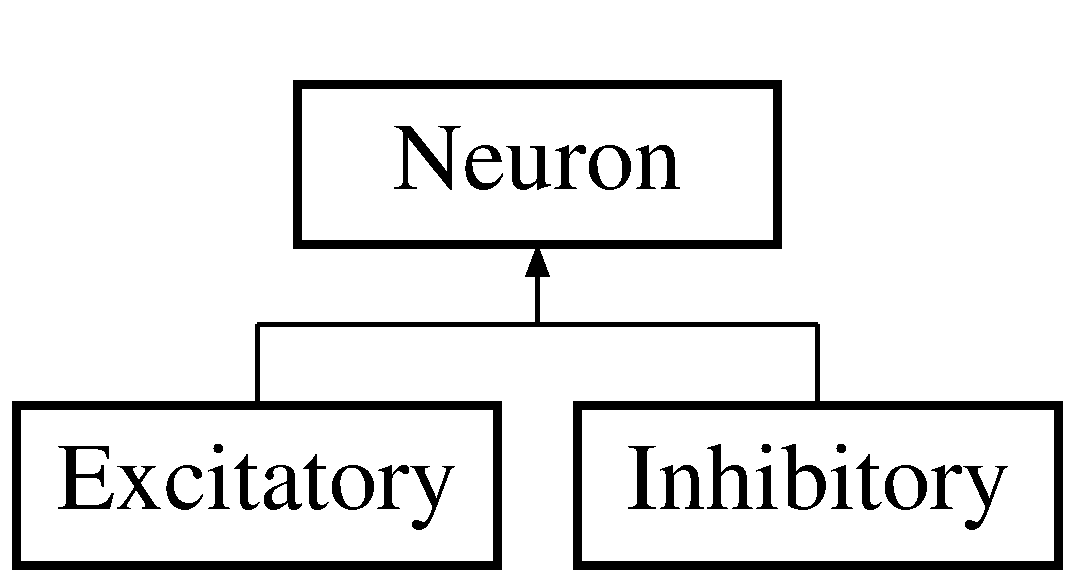
\includegraphics[height=2.000000cm]{class_neuron}
\end{center}
\end{figure}
\subsection*{Public Member Functions}
\begin{DoxyCompactItemize}
\item 
\textbf{ Neuron} (unsigned int index, double J, double V=0.\+0)
\item 
double \textbf{ get\+Potential} () const
\item 
double \textbf{ get\+Resistance} () const
\item 
double \textbf{ get\+Weight} () const
\item 
double \textbf{ get\+Delay} () const
\item 
unsigned int \textbf{ get\+Index} () const
\item 
unsigned int \textbf{ get\+Spikes\+Number} () const
\item 
std\+::vector$<$ double $>$ \textbf{ get\+Spikes\+Time} () const
\item 
void \textbf{ set\+Potential} (double V)
\item 
void \textbf{ receive\+\_\+spikes} (double J)
\item 
bool \textbf{ is\+Refractory} ()
\item 
bool \textbf{ update} (double I, unsigned int time)
\end{DoxyCompactItemize}
\subsection*{Static Public Attributes}
\begin{DoxyCompactItemize}
\item 
static constexpr unsigned int \textbf{ Ce\+\_\+} =10
\item 
static constexpr unsigned int \textbf{ Ci\+\_\+} =2
\item 
static constexpr double \textbf{ h\+\_\+} =0.\+1
\end{DoxyCompactItemize}


\subsection{Detailed Description}
The \doxyref{Neuron}{p.}{class_neuron} class 

\subsection{Constructor \& Destructor Documentation}
\mbox{\label{class_neuron_a5d32236ac46d84871e5884b6feb30194}} 
\index{Neuron@{Neuron}!Neuron@{Neuron}}
\index{Neuron@{Neuron}!Neuron@{Neuron}}
\subsubsection{Neuron()}
{\footnotesize\ttfamily Neuron\+::\+Neuron (\begin{DoxyParamCaption}\item[{unsigned int}]{index,  }\item[{double}]{J,  }\item[{double}]{V = {\ttfamily 0.0} }\end{DoxyParamCaption})}

Constructor 
\begin{DoxyParams}{Parameters}
{\em index} & the index of the neuron going from 0 to nb\+\_\+neurons-\/1(12500-\/1) \\
\hline
{\em J} & the amplitude of the postsynaptic current 0.\+1 mV for the excitatory neurons, 0.\+5 for the inhibitory \\
\hline
{\em V} & the membrane potential of the neuron in mV, bydefault initialisation of the membrane potential V\+\_\+ at 0.\+0 mV\\
\hline
\end{DoxyParams}
Constructor At the beggining of the simulation, the neurons have not yet received a postsynaptic current -\/$>$Every compartment of incoming\+\_\+spikes\+\_\+ should equal 0.\+0

To be sure that when we create a neuron, it has got not spike time

\subsection{Member Function Documentation}
\mbox{\label{class_neuron_aa1c3d933b84d2fdc60231c27f2075d82}} 
\index{Neuron@{Neuron}!get\+Delay@{get\+Delay}}
\index{get\+Delay@{get\+Delay}!Neuron@{Neuron}}
\subsubsection{get\+Delay()}
{\footnotesize\ttfamily double Neuron\+::get\+Delay (\begin{DoxyParamCaption}{ }\end{DoxyParamCaption}) const}

\begin{DoxyReturn}{Returns}
D\+\_\+ the delay of transmission between one neuron and his targets 
\end{DoxyReturn}
\mbox{\label{class_neuron_a2ebcd701dfaa9e9c20b601298f28097a}} 
\index{Neuron@{Neuron}!get\+Index@{get\+Index}}
\index{get\+Index@{get\+Index}!Neuron@{Neuron}}
\subsubsection{get\+Index()}
{\footnotesize\ttfamily unsigned int Neuron\+::get\+Index (\begin{DoxyParamCaption}{ }\end{DoxyParamCaption}) const}

\begin{DoxyReturn}{Returns}
index\+\_\+ the index of the neuron, between 0 and nb\+\_\+neurons-\/1(12500-\/1) 
\end{DoxyReturn}
\mbox{\label{class_neuron_acf44c8e2b57be445c2d802094a0c4f10}} 
\index{Neuron@{Neuron}!get\+Potential@{get\+Potential}}
\index{get\+Potential@{get\+Potential}!Neuron@{Neuron}}
\subsubsection{get\+Potential()}
{\footnotesize\ttfamily double Neuron\+::get\+Potential (\begin{DoxyParamCaption}{ }\end{DoxyParamCaption}) const}

Getters\begin{DoxyReturn}{Returns}
V\+\_\+ the membrane potential in mV
\end{DoxyReturn}
Getters \mbox{\label{class_neuron_ac2e50432a2f6d2400cc4cf0245dba573}} 
\index{Neuron@{Neuron}!get\+Resistance@{get\+Resistance}}
\index{get\+Resistance@{get\+Resistance}!Neuron@{Neuron}}
\subsubsection{get\+Resistance()}
{\footnotesize\ttfamily double Neuron\+::get\+Resistance (\begin{DoxyParamCaption}{ }\end{DoxyParamCaption}) const}

\begin{DoxyReturn}{Returns}
R\+\_\+ the membrane resistance 
\end{DoxyReturn}
\mbox{\label{class_neuron_ac3fef739c0da9a0ede8b5a1cc9338e2c}} 
\index{Neuron@{Neuron}!get\+Spikes\+Number@{get\+Spikes\+Number}}
\index{get\+Spikes\+Number@{get\+Spikes\+Number}!Neuron@{Neuron}}
\subsubsection{get\+Spikes\+Number()}
{\footnotesize\ttfamily unsigned int Neuron\+::get\+Spikes\+Number (\begin{DoxyParamCaption}{ }\end{DoxyParamCaption}) const}

\begin{DoxyReturn}{Returns}
spikes\+\_\+number\+\_\+ the number of time a neuron has spikes 
\end{DoxyReturn}
\mbox{\label{class_neuron_acefef3e7f04fce2db03a9589f6236ec0}} 
\index{Neuron@{Neuron}!get\+Spikes\+Time@{get\+Spikes\+Time}}
\index{get\+Spikes\+Time@{get\+Spikes\+Time}!Neuron@{Neuron}}
\subsubsection{get\+Spikes\+Time()}
{\footnotesize\ttfamily std\+::vector$<$ double $>$ Neuron\+::get\+Spikes\+Time (\begin{DoxyParamCaption}{ }\end{DoxyParamCaption}) const}

\begin{DoxyReturn}{Returns}
spikes\+\_\+time\+\_\+ the time of the spikes that have occurred 
\end{DoxyReturn}
\mbox{\label{class_neuron_a176485cd940e7dbf954d68e23477dbfb}} 
\index{Neuron@{Neuron}!get\+Weight@{get\+Weight}}
\index{get\+Weight@{get\+Weight}!Neuron@{Neuron}}
\subsubsection{get\+Weight()}
{\footnotesize\ttfamily double Neuron\+::get\+Weight (\begin{DoxyParamCaption}{ }\end{DoxyParamCaption}) const}

\begin{DoxyReturn}{Returns}
J\+\_\+ the amplitude of the postsynaptic current 
\end{DoxyReturn}
\mbox{\label{class_neuron_a8a86e93b1619baf27aaf1dd1ff9fc799}} 
\index{Neuron@{Neuron}!is\+Refractory@{is\+Refractory}}
\index{is\+Refractory@{is\+Refractory}!Neuron@{Neuron}}
\subsubsection{is\+Refractory()}
{\footnotesize\ttfamily bool Neuron\+::is\+Refractory (\begin{DoxyParamCaption}{ }\end{DoxyParamCaption})}

\begin{DoxyReturn}{Returns}
true if the neuron is in a refractory period 
\end{DoxyReturn}
check if it has already spiked, otherwise it cannot be in the refractory period

check if the current time -\/ the last spike time is smaller than the refractory period\mbox{\label{class_neuron_ab6509981d2a8518bb4b38d0a81e87849}} 
\index{Neuron@{Neuron}!receive\+\_\+spikes@{receive\+\_\+spikes}}
\index{receive\+\_\+spikes@{receive\+\_\+spikes}!Neuron@{Neuron}}
\subsubsection{receive\+\_\+spikes()}
{\footnotesize\ttfamily void Neuron\+::receive\+\_\+spikes (\begin{DoxyParamCaption}\item[{double}]{J }\end{DoxyParamCaption})}

The method receive\+\_\+spikes is used whenever a neuron that has targets spikes, it adds in the compartment corresponding to (delay\+\_\++clock\+\_\+)Dmax\+\_\+ of the buffer incoming\+\_\+spikes\+\_\+ the value of J 
\begin{DoxyParams}{Parameters}
{\em J} & the amplitude of the postsynaptic current 0.\+1mV for the excitatory and 0.\+5 mV for the inhibitory \\
\hline
\end{DoxyParams}
the amplitude of the postsynaptic current is added in the buffer\textquotesingle{}s compartment corresponding to (D\+\_\++clock\+\_\+)Dmax\+\_\+\mbox{\label{class_neuron_a1ca0aa5a828d37348023b51f31785c82}} 
\index{Neuron@{Neuron}!set\+Potential@{set\+Potential}}
\index{set\+Potential@{set\+Potential}!Neuron@{Neuron}}
\subsubsection{set\+Potential()}
{\footnotesize\ttfamily void Neuron\+::set\+Potential (\begin{DoxyParamCaption}\item[{double}]{V }\end{DoxyParamCaption})}

Setter set the membrane potential V\+\_\+ to a given value V

Setter \mbox{\label{class_neuron_a8495a3728f74b6bd7ce5b0e97ff7bda6}} 
\index{Neuron@{Neuron}!update@{update}}
\index{update@{update}!Neuron@{Neuron}}
\subsubsection{update()}
{\footnotesize\ttfamily bool Neuron\+::update (\begin{DoxyParamCaption}\item[{double}]{I,  }\item[{unsigned int}]{time }\end{DoxyParamCaption})}

update the neuron state from time t to time t+T, where T is n$\ast$h (h pas de temps) This method recalculates the mebrane potential at each step of time, except if the neuron is in his refractory period The membrane potential is calculated by (c1\+\_\+$\ast$\+V\+\_\++\+I$\ast$c2\+\_\++d(gen)) where d(gen) is a random value following a poisson distibution of (V\+\_\+ext\+\_\+$\ast$\+J\+\_\+$\ast$h\+\_\+ $\ast$\+Ce\+\_\+) It then adds, the postsynaptic current if there is one associated with the step of time \begin{DoxySeeAlso}{See also}
\doxyref{receive\+\_\+spikes(double J)}{p.}{class_neuron_ab6509981d2a8518bb4b38d0a81e87849} It verifies whether a neuron has spiked -\/$>$ if it has, spikes\+\_\+number\+\_\+ is incremented and spikes\+\_\+time\+\_\+ record the current time The personnal time of the neuron is finally incremented 
\end{DoxySeeAlso}

\begin{DoxyParams}{Parameters}
{\em I} & corresponds to the external current \\
\hline
{\em time} & corresponds to the simulation time \\
\hline
\end{DoxyParams}
\begin{DoxyReturn}{Returns}
true if the neuron has spiked
\end{DoxyReturn}
Update If neuron is refractory -\/$>$ neuron has spiked -\/$>$ V will not be modified

Creation of a random device

The random generator follows a poisson distribution with λ = V\+\_\+ext\+\_\+$\ast$\+J\+\_\+$\ast$h\+\_\+ $\ast$\+Ce\+\_\+

The external current I is equal to 0

If a spike is associated with the current time, we add it to the new potential

Reinitialisation of the value of my buffer corresponding to the compartment [clockDmax] that have just been used

A spike occurres if the membrane potential is greater than the membrane potential threshold

After a spike, the potential gets back to its reset value

Modifies the attribute membrane potential V\+\_\+

The local clock of my neuron is incremented at the end of the update

\subsection{Member Data Documentation}
\mbox{\label{class_neuron_a6c9869121fb7ac15aadd3e6059f6dd11}} 
\index{Neuron@{Neuron}!Ce\+\_\+@{Ce\+\_\+}}
\index{Ce\+\_\+@{Ce\+\_\+}!Neuron@{Neuron}}
\subsubsection{Ce\+\_\+}
{\footnotesize\ttfamily constexpr unsigned int Neuron\+::\+Ce\+\_\+ =10\hspace{0.3cm}{\ttfamily [static]}}

public static attributs of the class \doxyref{Neuron}{p.}{class_neuron} Do not change from one neurons to another and need to be accessed from outside the class -\/$>$ no getter because static method should not be constant\+Ce\+\_\+ = Number of excitatory connexion of one neuron -\/$>$ 1000 \mbox{\label{class_neuron_a22b5ca4f7064fcd2a451a1336242f91e}} 
\index{Neuron@{Neuron}!Ci\+\_\+@{Ci\+\_\+}}
\index{Ci\+\_\+@{Ci\+\_\+}!Neuron@{Neuron}}
\subsubsection{Ci\+\_\+}
{\footnotesize\ttfamily constexpr unsigned int Neuron\+::\+Ci\+\_\+ =2\hspace{0.3cm}{\ttfamily [static]}}

Ci\+\_\+ = Number of excitatory connexion of one neuron -\/$>$ 250 \mbox{\label{class_neuron_a17c11789cb4caff4ec075a81adc0d3eb}} 
\index{Neuron@{Neuron}!h\+\_\+@{h\+\_\+}}
\index{h\+\_\+@{h\+\_\+}!Neuron@{Neuron}}
\subsubsection{h\+\_\+}
{\footnotesize\ttfamily constexpr double Neuron\+::h\+\_\+ =0.\+1\hspace{0.3cm}{\ttfamily [static]}}

h = step of time in 0.\+1 ms 

The documentation for this class was generated from the following files\+:\begin{DoxyCompactItemize}
\item 
Neuron.\+hpp\item 
Neuron.\+cpp\end{DoxyCompactItemize}

%--- End generated contents ---

% Index
\backmatter
\newpage
\phantomsection
\clearemptydoublepage
\addcontentsline{toc}{chapter}{Index}
\printindex

\end{document}
